% Created by tikzDevice version 0.12 on 2018-09-20 18:19:33
% !TEX encoding = UTF-8 Unicode
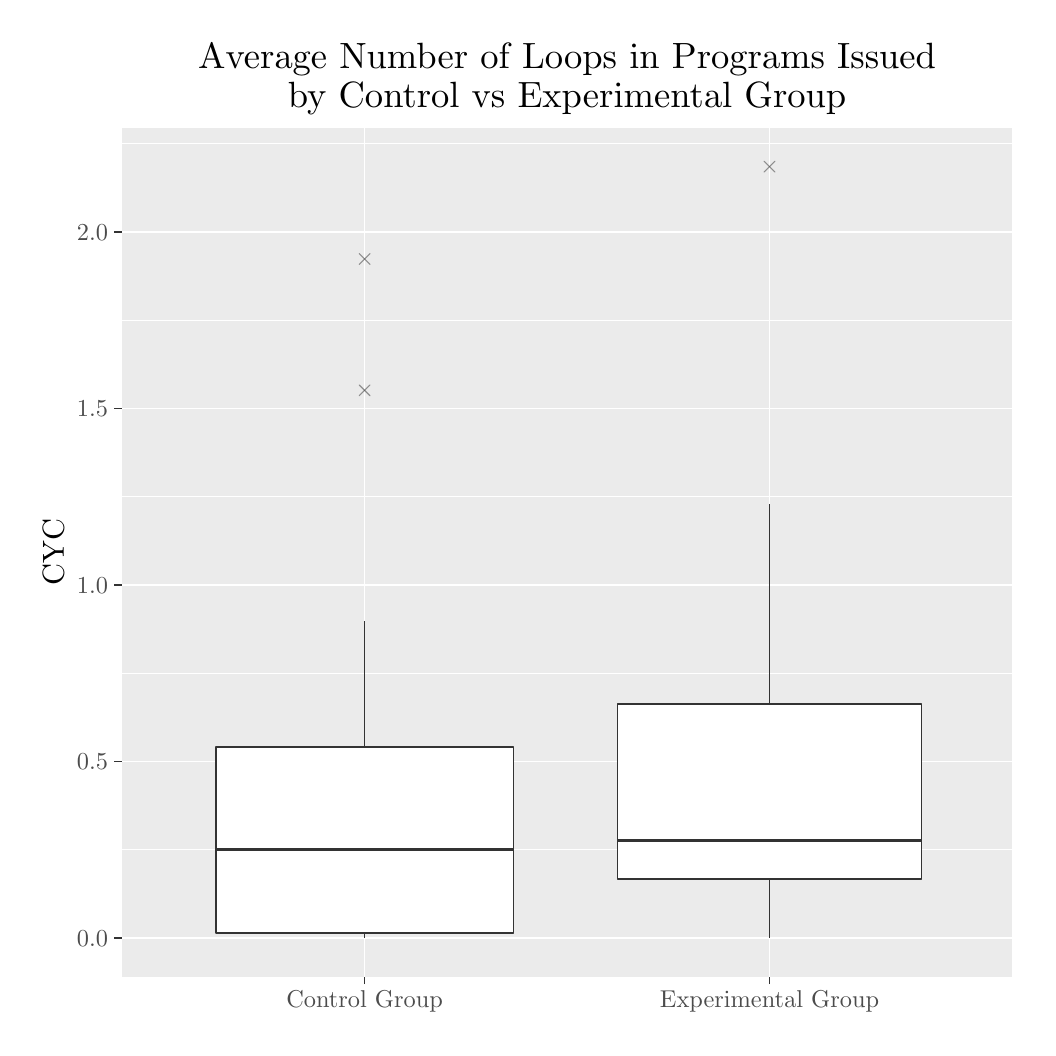
\begin{tikzpicture}[x=1pt,y=1pt]
\definecolor{fillColor}{RGB}{255,255,255}
\path[use as bounding box,fill=fillColor,fill opacity=0.00] (0,0) rectangle (361.35,361.35);
\begin{scope}
\path[clip] (  0.00,  0.00) rectangle (361.35,361.35);
\definecolor{drawColor}{RGB}{255,255,255}
\definecolor{fillColor}{RGB}{255,255,255}

\path[draw=drawColor,line width= 0.6pt,line join=round,line cap=round,fill=fillColor] (  0.00,  0.00) rectangle (361.35,361.35);
\end{scope}
\begin{scope}
\path[clip] ( 33.96, 18.45) rectangle (355.85,325.06);
\definecolor{fillColor}{gray}{0.92}

\path[fill=fillColor] ( 33.96, 18.45) rectangle (355.85,325.06);
\definecolor{drawColor}{RGB}{255,255,255}

\path[draw=drawColor,line width= 0.3pt,line join=round] ( 33.96, 64.28) --
	(355.85, 64.28);

\path[draw=drawColor,line width= 0.3pt,line join=round] ( 33.96,128.05) --
	(355.85,128.05);

\path[draw=drawColor,line width= 0.3pt,line join=round] ( 33.96,191.82) --
	(355.85,191.82);

\path[draw=drawColor,line width= 0.3pt,line join=round] ( 33.96,255.59) --
	(355.85,255.59);

\path[draw=drawColor,line width= 0.3pt,line join=round] ( 33.96,319.36) --
	(355.85,319.36);

\path[draw=drawColor,line width= 0.6pt,line join=round] ( 33.96, 32.39) --
	(355.85, 32.39);

\path[draw=drawColor,line width= 0.6pt,line join=round] ( 33.96, 96.16) --
	(355.85, 96.16);

\path[draw=drawColor,line width= 0.6pt,line join=round] ( 33.96,159.93) --
	(355.85,159.93);

\path[draw=drawColor,line width= 0.6pt,line join=round] ( 33.96,223.71) --
	(355.85,223.71);

\path[draw=drawColor,line width= 0.6pt,line join=round] ( 33.96,287.48) --
	(355.85,287.48);

\path[draw=drawColor,line width= 0.6pt,line join=round] (121.75, 18.45) --
	(121.75,325.06);

\path[draw=drawColor,line width= 0.6pt,line join=round] (268.06, 18.45) --
	(268.06,325.06);
\definecolor{drawColor}{RGB}{51,51,51}

\path[draw=drawColor,draw opacity=0.50,line width= 0.4pt,line join=round,line cap=round] (266.10,309.16) -- (270.02,313.08);

\path[draw=drawColor,draw opacity=0.50,line width= 0.4pt,line join=round,line cap=round] (266.10,313.08) -- (270.02,309.16);
\definecolor{drawColor}{gray}{0.20}

\path[draw=drawColor,line width= 0.6pt,line join=round] (268.06,117.05) -- (268.06,189.30);

\path[draw=drawColor,line width= 0.6pt,line join=round] (268.06, 53.68) -- (268.06, 32.39);
\definecolor{fillColor}{RGB}{255,255,255}

\path[draw=drawColor,line width= 0.6pt,line join=round,line cap=round,fill=fillColor] (213.19,117.05) --
	(213.19, 53.68) --
	(322.93, 53.68) --
	(322.93,117.05) --
	(213.19,117.05) --
	cycle;

\path[draw=drawColor,line width= 1.1pt,line join=round] (213.19, 67.75) -- (322.93, 67.75);
\definecolor{drawColor}{RGB}{51,51,51}

\path[draw=drawColor,draw opacity=0.50,line width= 0.4pt,line join=round,line cap=round] (119.79,275.79) -- (123.71,279.71);

\path[draw=drawColor,draw opacity=0.50,line width= 0.4pt,line join=round,line cap=round] (119.79,279.71) -- (123.71,275.79);

\path[draw=drawColor,draw opacity=0.50,line width= 0.4pt,line join=round,line cap=round] (119.79,228.34) -- (123.71,232.26);

\path[draw=drawColor,draw opacity=0.50,line width= 0.4pt,line join=round,line cap=round] (119.79,232.26) -- (123.71,228.34);
\definecolor{drawColor}{gray}{0.20}

\path[draw=drawColor,line width= 0.6pt,line join=round] (121.75,101.33) -- (121.75,146.96);

\path[draw=drawColor,line width= 0.6pt,line join=round] (121.75, 34.14) -- (121.75, 32.39);

\path[draw=drawColor,line width= 0.6pt,line join=round,line cap=round,fill=fillColor] ( 67.95,101.33) --
	( 67.95, 34.14) --
	(175.55, 34.14) --
	(175.55,101.33) --
	( 67.95,101.33) --
	cycle;

\path[draw=drawColor,line width= 1.1pt,line join=round] ( 67.95, 64.28) -- (175.55, 64.28);
\end{scope}
\begin{scope}
\path[clip] (  0.00,  0.00) rectangle (361.35,361.35);
\definecolor{drawColor}{gray}{0.30}

\node[text=drawColor,anchor=base east,inner sep=0pt, outer sep=0pt, scale=  0.88] at ( 29.01, 29.36) {0.0};

\node[text=drawColor,anchor=base east,inner sep=0pt, outer sep=0pt, scale=  0.88] at ( 29.01, 93.13) {0.5};

\node[text=drawColor,anchor=base east,inner sep=0pt, outer sep=0pt, scale=  0.88] at ( 29.01,156.90) {1.0};

\node[text=drawColor,anchor=base east,inner sep=0pt, outer sep=0pt, scale=  0.88] at ( 29.01,220.68) {1.5};

\node[text=drawColor,anchor=base east,inner sep=0pt, outer sep=0pt, scale=  0.88] at ( 29.01,284.45) {2.0};
\end{scope}
\begin{scope}
\path[clip] (  0.00,  0.00) rectangle (361.35,361.35);
\definecolor{drawColor}{gray}{0.20}

\path[draw=drawColor,line width= 0.6pt,line join=round] ( 31.21, 32.39) --
	( 33.96, 32.39);

\path[draw=drawColor,line width= 0.6pt,line join=round] ( 31.21, 96.16) --
	( 33.96, 96.16);

\path[draw=drawColor,line width= 0.6pt,line join=round] ( 31.21,159.93) --
	( 33.96,159.93);

\path[draw=drawColor,line width= 0.6pt,line join=round] ( 31.21,223.71) --
	( 33.96,223.71);

\path[draw=drawColor,line width= 0.6pt,line join=round] ( 31.21,287.48) --
	( 33.96,287.48);
\end{scope}
\begin{scope}
\path[clip] (  0.00,  0.00) rectangle (361.35,361.35);
\definecolor{drawColor}{gray}{0.20}

\path[draw=drawColor,line width= 0.6pt,line join=round] (121.75, 15.70) --
	(121.75, 18.45);

\path[draw=drawColor,line width= 0.6pt,line join=round] (268.06, 15.70) --
	(268.06, 18.45);
\end{scope}
\begin{scope}
\path[clip] (  0.00,  0.00) rectangle (361.35,361.35);
\definecolor{drawColor}{gray}{0.30}

\node[text=drawColor,anchor=base,inner sep=0pt, outer sep=0pt, scale=  0.88] at (121.75,  7.44) {Control Group};

\node[text=drawColor,anchor=base,inner sep=0pt, outer sep=0pt, scale=  0.88] at (268.06,  7.44) {Experimental Group};
\end{scope}
\begin{scope}
\path[clip] (  0.00,  0.00) rectangle (361.35,361.35);
\definecolor{drawColor}{RGB}{0,0,0}

\node[text=drawColor,rotate= 90.00,anchor=base,inner sep=0pt, outer sep=0pt, scale=  1.10] at ( 13.08,171.76) {CYC};
\end{scope}
\begin{scope}
\path[clip] (  0.00,  0.00) rectangle (361.35,361.35);
\definecolor{drawColor}{RGB}{0,0,0}

\node[text=drawColor,anchor=base,inner sep=0pt, outer sep=0pt, scale=  1.32] at (194.91,346.76) {Average Number of Loops in Programs Issued};

\node[text=drawColor,anchor=base,inner sep=0pt, outer sep=0pt, scale=  1.32] at (194.91,332.50) {by Control vs Experimental Group};
\end{scope}
\end{tikzpicture}
